% Editable task illustration. Examples are manually written, not predictions.
\begin{tikzpicture}[x=1cm,y=1cm]
\node[fllabel,anchor=west] at (0,2.7) {输入：单张餐食 RGB 图像};
\node[inner sep=0] (meal) at (2.35,.1)
 {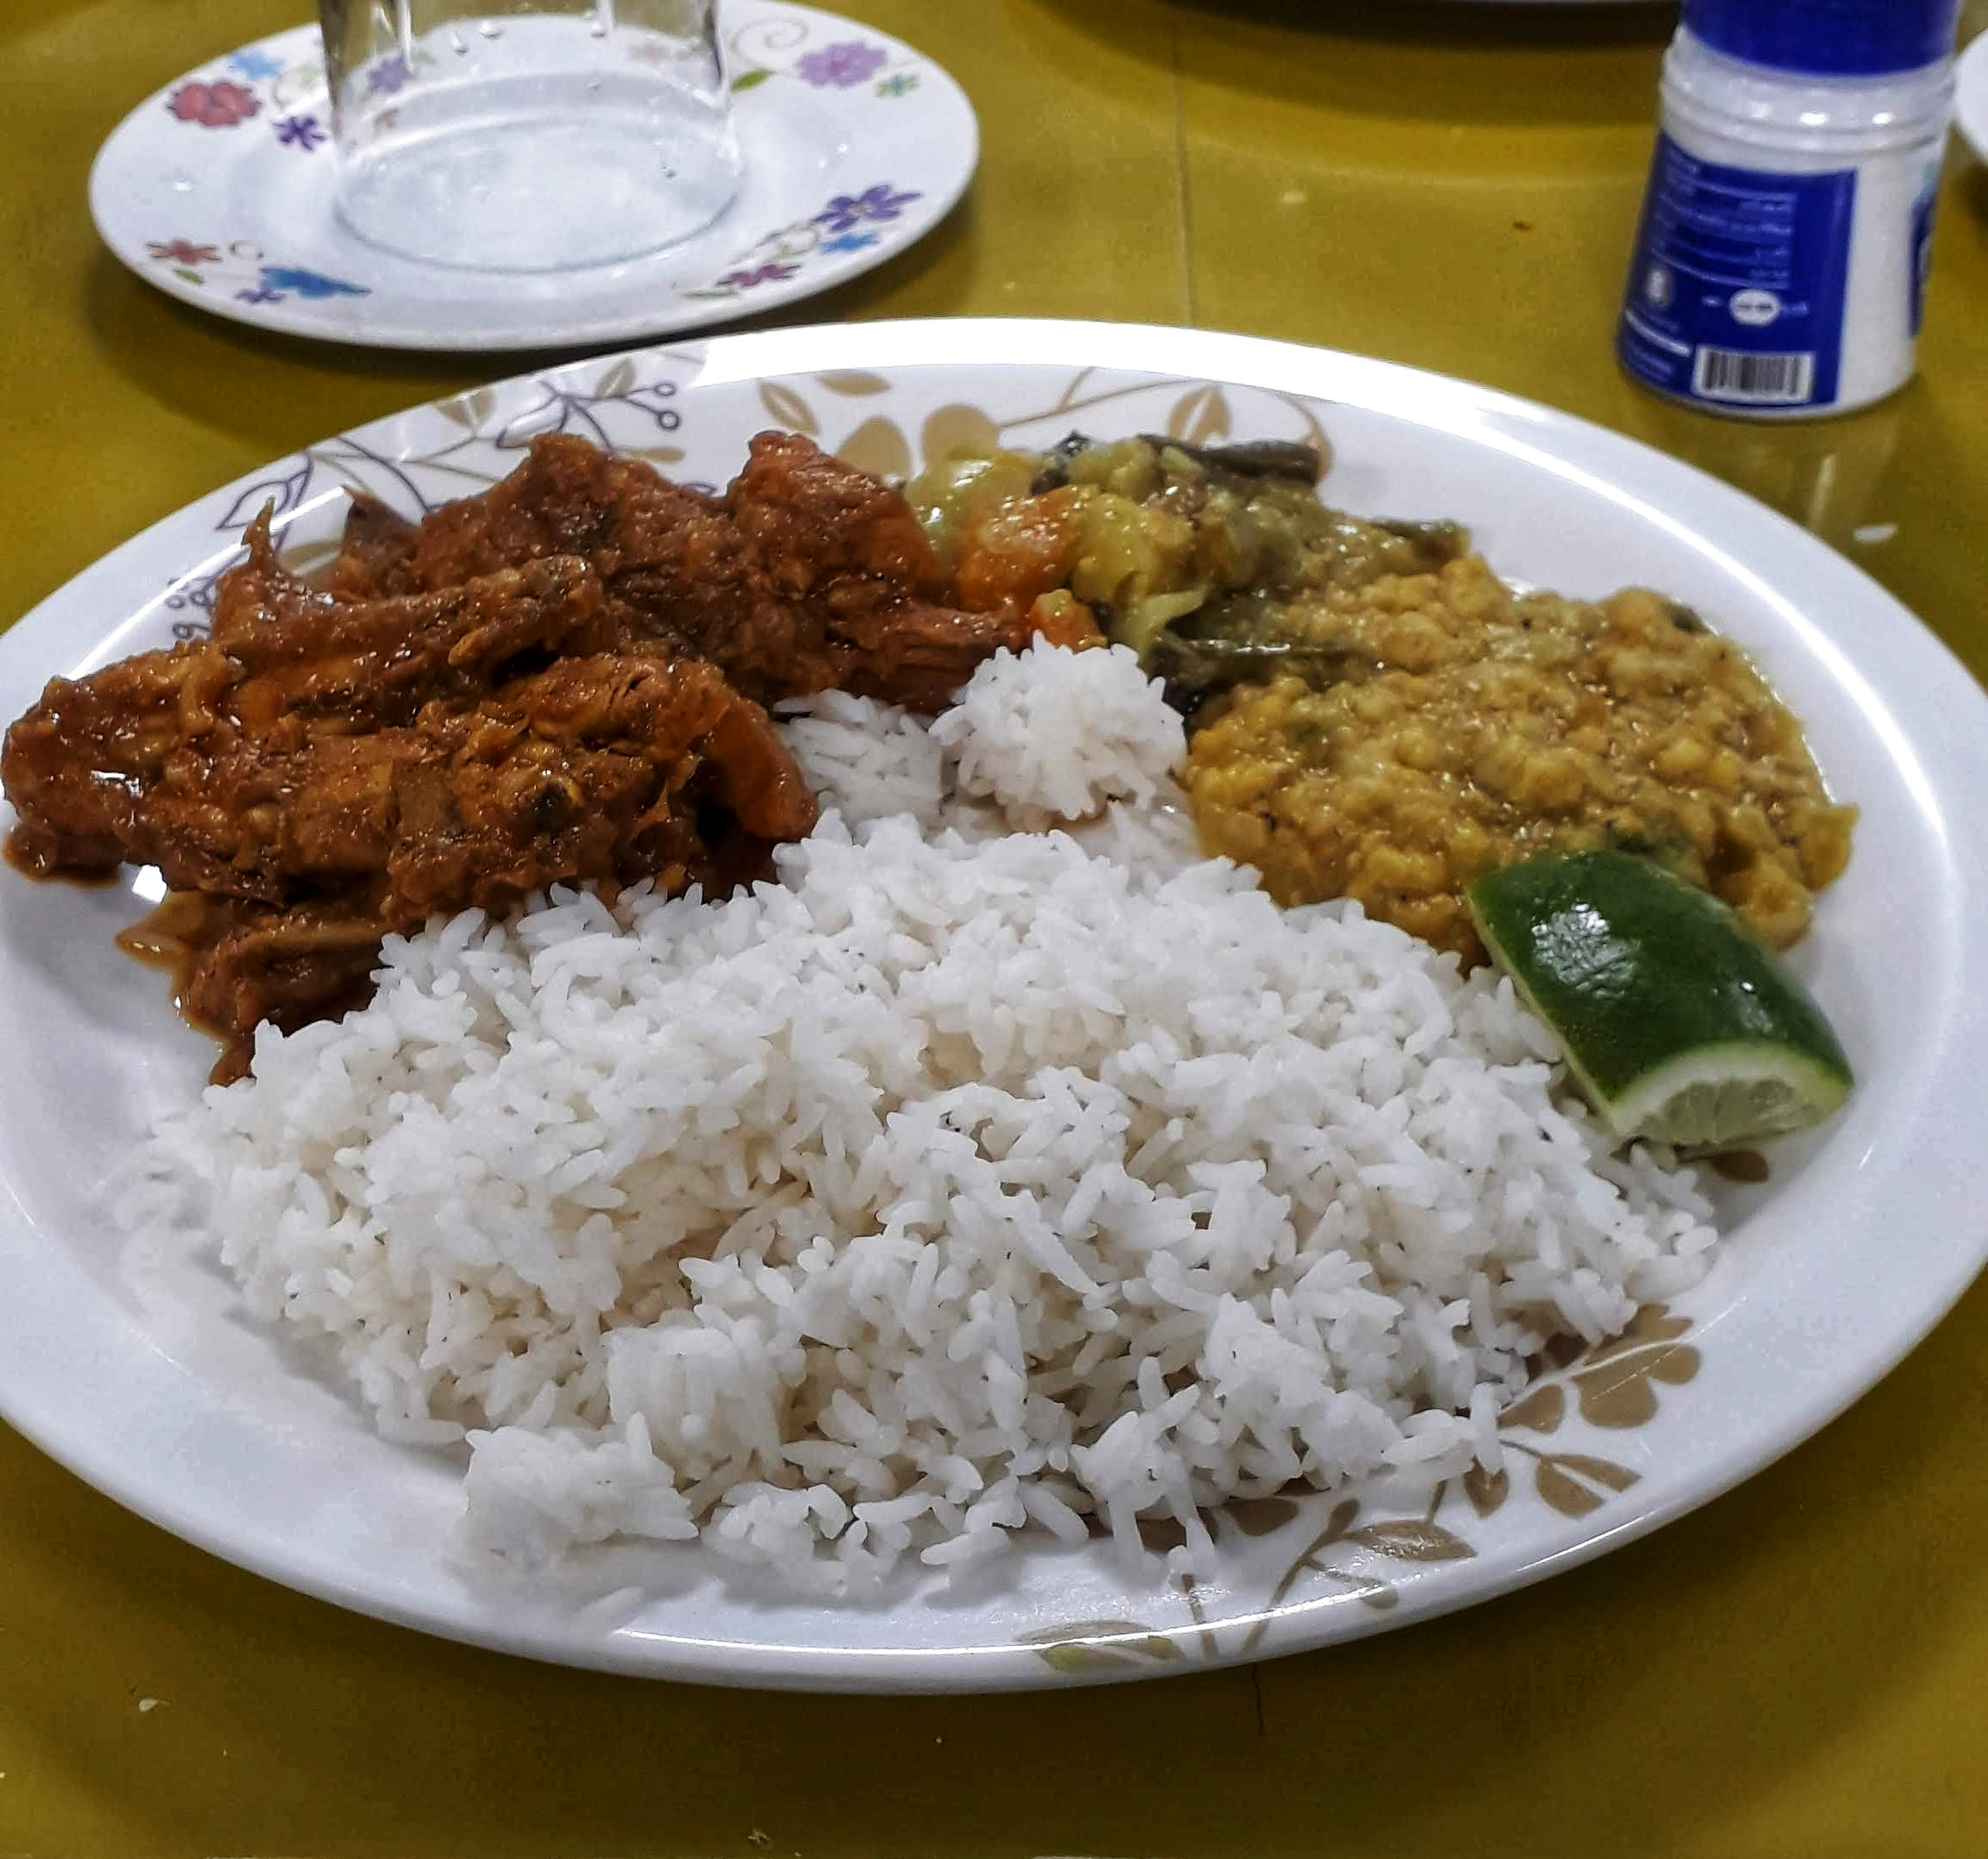
\includegraphics[width=4.6cm]{figures/context/meal_platter.jpg}};
\node[flnote,text width=4.6cm] at (2.35,-2.4) {可见食物与外观提供视觉线索\\实际重量和营养需要估计};

\node[fltrain,anchor=north west,text width=8.7cm,align=left,inner sep=8pt] (caption) at (6.0,2.9)
 {\textbf{\color{FLBlue}任务一 · 英文描述示例}\\[4pt]
 A plate of white rice with several side dishes.};
\node[flaccent,anchor=north west,text width=8.7cm,align=left,inner sep=8pt] (record) at (6.0,1.15)
 {\textbf{\color{FLBlue}任务二 · JSON 字段示例}\\[4pt]
 {\ttfamily\fontsize{8.5}{10.5}\selectfont
 \{\\
 \hspace*{1em}"items": [\{"name": "rice", "weight\_g": null\}],\\
 \hspace*{1em}"total\_weight\_g": null,\\
 \hspace*{1em}"total\_calories\_kcal": null,\\
 \hspace*{1em}"protein\_g": null,\\
 \hspace*{1em}"fat\_g": null,\\
 \hspace*{1em}"carbohydrate\_g": null\\
 \}}\\[4pt]
 {\fontsize{8}{10}\selectfont\color{FLMid}仅列一项食材；null 表示待估，实际输出须为数值。}};
\draw[flarrow] (4.72,.95) -- ++(.55,0) |- (caption.west);
\draw[flarrow] (4.72,-.6) -- ++(.55,0) |- (record.west);

\draw[FLLine,dashed] (0,-3.65)--(15.25,-3.65);
\node[fllabel,anchor=west] at (0,-4.0) {训练衔接：描述模型如何成为 Hybrid};
\node[flnode,text width=3.7cm,minimum height=.85cm] (source) at (2.05,-4.85)
 {任务一训练好的模型 A\\图像描述能力};
\node[flaccent,text width=4.65cm,minimum height=.85cm] (transfer) at (7.6,-4.85)
 {迁移视觉编码器与 GRU\\新增重量、营养回归头};
\node[fltrain,text width=3.7cm,minimum height=.85cm] (hybrid) at (13.15,-4.85)
 {任务二数据联合训练\\得到 Hybrid 模型};
\draw[flarrow] (source.east)--(transfer.west);
\draw[flarrow] (transfer.east)--(hybrid.west);
\end{tikzpicture}

